\documentclass{article}
\usepackage[brazilian]{babel}
\usepackage[utf8]{inputenc}
\usepackage[T1]{fontenc}
\usepackage{listings}
\usepackage{xcolor}
\usepackage{graphicx}
\usepackage{geometry}

\definecolor{darkgreen}{rgb}{0,0.5,0}

\geometry{
  a4paper,
  total={170mm,257mm},
  left=25mm,
  top=20mm,
  }

\graphicspath{ {./images/} }


\lstset{language=C++,
basicstyle=\ttfamily\small,
keywordstyle=\color{blue}\ttfamily,
stringstyle=\color{red}\ttfamily,
commentstyle=\color{darkgreen}\ttfamily
}

\author{
  Mauricio Ramos Ribeiro\\
  \texttt{mauricio.ribeiro@outlook.com.br}
}


\title{Respostas do Exercício de Ordenacao}
\date{\today}

\begin{document}
\maketitle

\vspace{15mm}


\section*{Questão 1:}
\lstinputlisting[language=C++, firstline=1]{../extra/ordena2.cpp}
\begin{figure}[h!]
  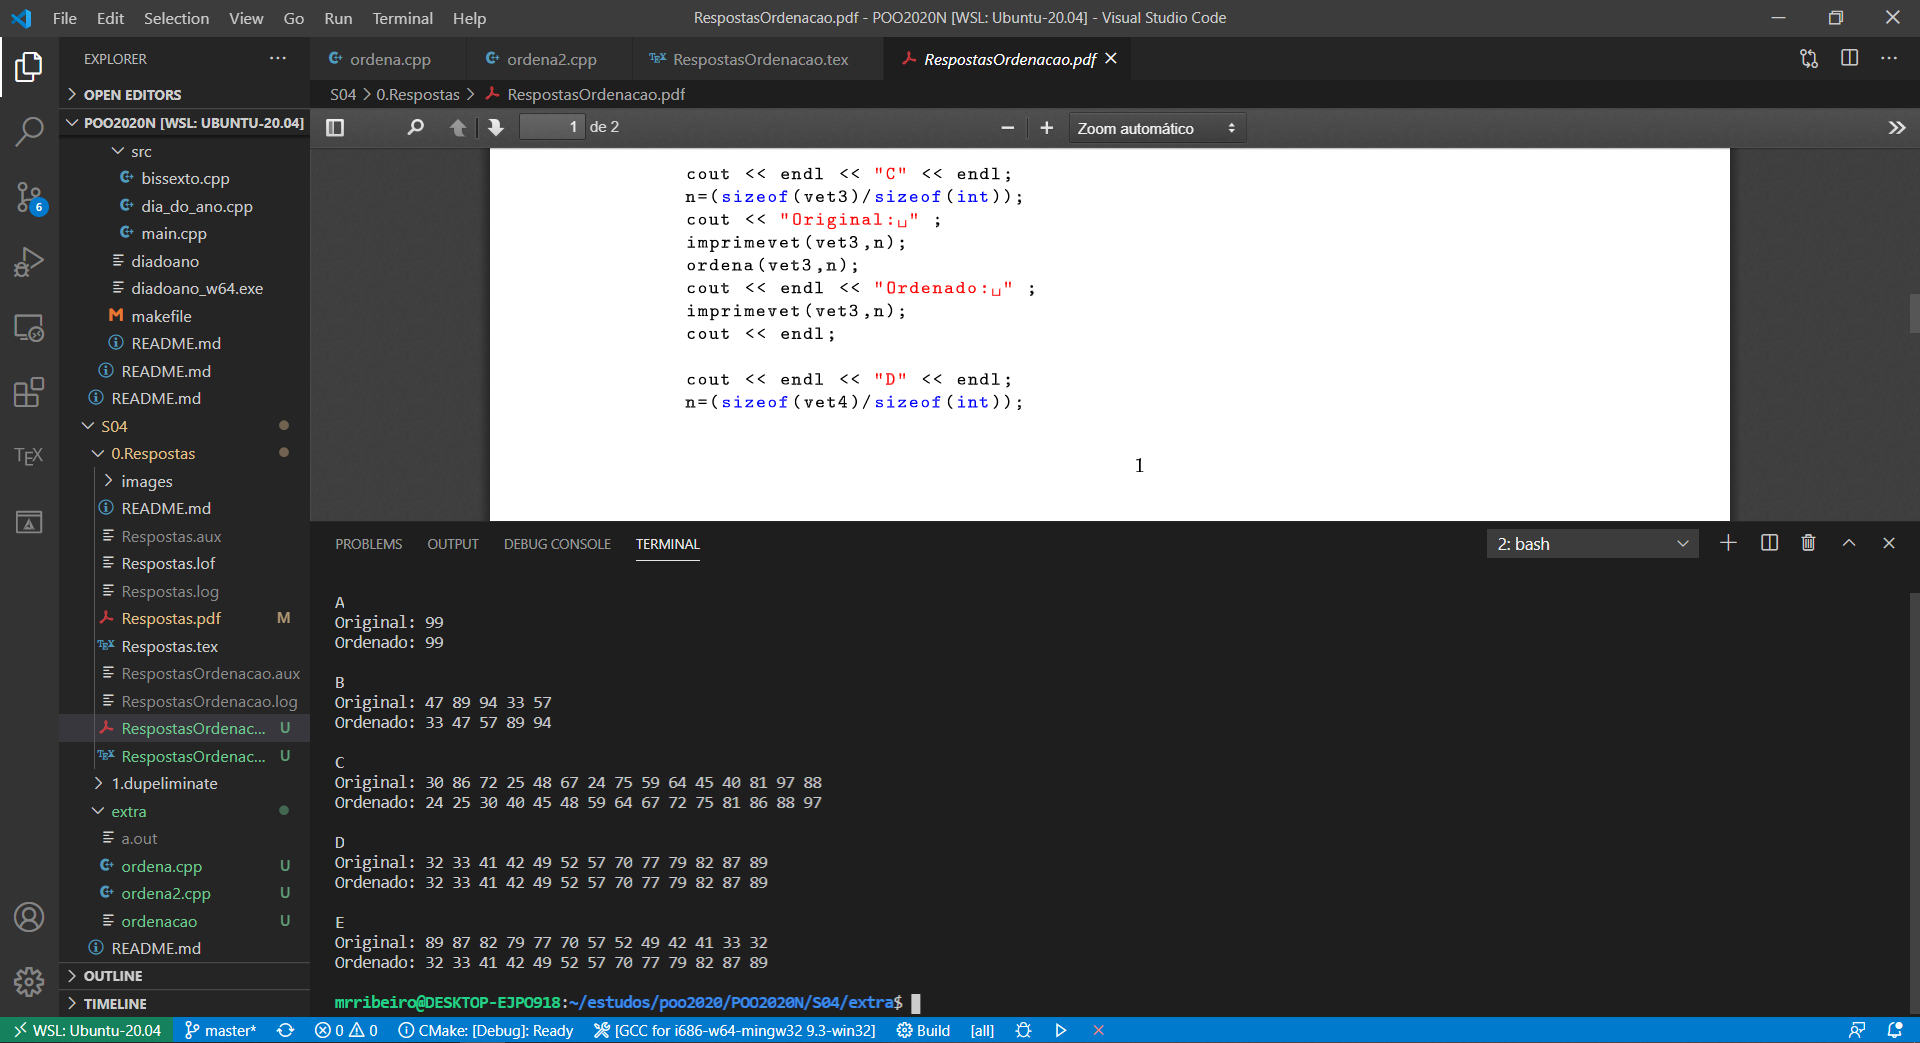
\includegraphics[scale=0.5]{Extra01.png}
  \caption{Execução do Código da Questão 1}
\end{figure}

\vspace{15mm}




\end{document}